\documentclass[conference]{IEEEtran}

\usepackage[utf8]{inputenc}
\usepackage{amsmath}
\usepackage{units}
\usepackage{graphicx}
\usepackage{multirow}
\usepackage{comment}
\usepackage{listings}
\usepackage{placeins}
\usepackage{float}
\usepackage{hyperref}

\begin{document}
\title{An Ensemble Approach using Convolution and Recurrent Neural Networks for Human Action Recognition on the UTD-MHAD}

\author{\IEEEauthorblockN{Tan Ren Jie\IEEEauthorrefmark{1},
Kelvin Yeo Ngan Chong\IEEEauthorrefmark{2}, and Khaing Mon Kyaw\IEEEauthorrefmark{3} } \\
\IEEEauthorblockA{Institute of Systems Science, National University of Singapore \\
Email: e0267395@u.nus.edu\IEEEauthorrefmark{1},
e0267573@u.nus.edu\IEEEauthorrefmark{2},
e0146800@u.nus.edu\IEEEauthorrefmark{3},
}}
\maketitle

\begin{abstract}
In this paper, we shall demonstrate an ensemble approach of performing Human Action Recognition on the University of Texas at Dallas Multimodal Human Action Dataset(UTD-MHAD), which comprises of $27$ different human actions. The ensemble approach gained an accuracy of $0.821$ on the validation data, which is a significant improvement to the baseline paper's accuracy of $0.672$. The paper also shows the train-val performances of other models we experimented using only the Inertial and Skeleton dataset. The link to Github repository which holds to code can be found \href{https://github.com/notha99y/Multimodal_human_actions}{here}, and the link to get the dataset can be found \href{https://www.utdallas.edu/~kehtar/UTD-MHAD.html}{here}.
\end{abstract}

\section{Introduction}
Human Action Recognition (HAR) has been a research field that piqued interests from several computer science communities since the 1980s, due to its application in many different fields of study, such as medicine, human-computer interaction, sociology. Data in the format of videos, inertial sensors, like accelerometers  and gyroscopes, depth maps and point clouds are often used to classify the different human actions \cite{4487086}\cite{7881728}. \\ \\
Traditional approaches can be generally broken down into the following 3 steps:
\begin{enumerate}
\item Feature Extraction using Signal Processing or Computer Vision techniques to capture relevant spatio-temporal features \cite{5995407}\cite{1238378}\cite{1570899}
\item Designing a pipeline to combine the extracted features 
\item Training a classifier, usually a Support Vector Machine (SVM) or Random Forest (RF), using these features  
\end{enumerate}
\vspace{0.5cm}
This approach often requires deep domain knowledge in extracting the useful spatio-temporal features. Another approach is to use modern neural network architectures to do the feature extraction and model building automatically. Soon after $2014$, there were two breakthrough papers, Single Stream and Two Stream, which ignited the research using modern approach. The main difference between them was how the model architecture combines the spatio-temporal information. \\ \\
The first paper \cite{KarpathyCVPR14} uses a 
Single Stream Network which explores various ways to fuse temporal information from consecutive frames using 2D pre-trained convolutions. This had led to popular methods such as Long-term Recurrent Convolutional Networks (LRCN) \cite{DonahueHGRVSD14},
3-D Convolutional Networks \cite{TranBFTP14}, and 
Conv3D with Attention \cite{YaoTCBPLC}. \\ \\
The second paper uses a Two Stream Network \cite{SimonyanZ14}, as shown in Fig. \ref{fig:twostreamarchi}, one stream captures the spatial context (pre-trained), while the other captures the motion context. Other variants are soon developed as like the 
Two-Stream Network Fusion \cite{FeichtenhoferPZ16}, Temporal Segment Networks (TSN) \cite{WangXW0LTG16},
Action Video-Level Aggregation (ActionVLAD) \cite{GirdharRGSR17},
Hidden Two-Stream Convolutional Networks \cite{ZhuLNH17a},
Two-Stream Inflated 3D ConvNet (Two-StreamI3D) \cite{CarreiraZ17}, and Temporal 3D ConvNets (T3D) \cite{AliMVAMRL} \\ 
\begin{figure}[H]
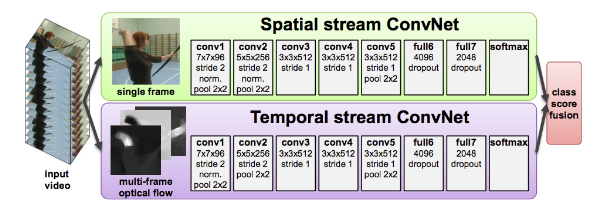
\includegraphics[scale=0.4]{two_stream_architecture.png}
\caption{\label{fig:twostreamarchi} Two stream architecture proposed by Simmoyan and Zisserman \cite{SimonyanZ14}}
\end{figure}
In this paper, we shall present an ensemble approach, using both convolutional and recurrent, single stream neural networks to recognize 27 different human actions using the UTD-MHAD dataset \cite{UTD-MHAD}. 
\section{Methods and Modeling}
\subsection{Dataset}
Collected via a Microsoft Kinect sensor, a wearable inertial sensor, which includes an accelerometer and a gyroscope, and video camera, the UTD-MHAD dataset contains 27 different actions performed by 8 subjects (4 females and 4 males). Each subject was asked to repeat each action 4 times. After removing three corrupted sequences, the dataset contains 861 sequences. There are 4 different types of data, the Depth dataset, Inertial dataset, Skeleton dataset, and RGB dataset. They are plotted and shown respectively in Fig. \ref{fig:tennis_swing_depth} - \ref{fig:tennis_swing_vid}.
\begin{figure}[H]
\begin{center}
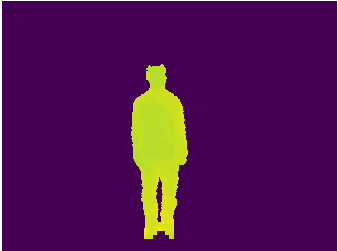
\includegraphics[scale=0.3]{depth_tennis_swing.png}
\caption{\label{fig:tennis_swing_depth} Depth map dataset of a subject performing a tennis swing}
\end{center}
\end{figure}
\begin{figure}[H]
\begin{center}
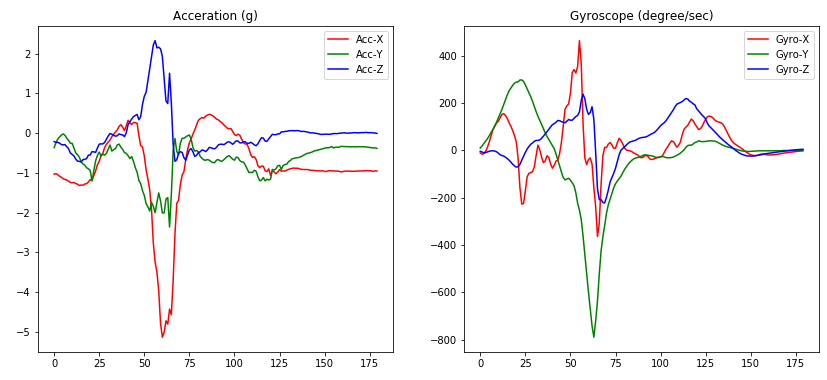
\includegraphics[scale=0.3]{inertial_tennis_swing.png}
\end{center}
\caption{\label{fig:tennis_swing_iner} Inertial dataset of a subject performing a tennis swing}
\end{figure}
\begin{figure}[H]
\begin{center}
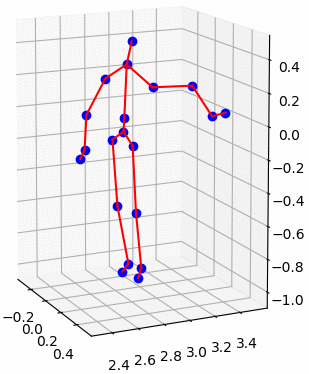
\includegraphics[scale=0.3]{skeleton_tennis_swing.png}
\end{center}
\caption{\label{fig:tennis_swing_skel} Skeleton dataset of a subject performing a tennis swing}
\end{figure}
\begin{figure}[H]
\begin{center}
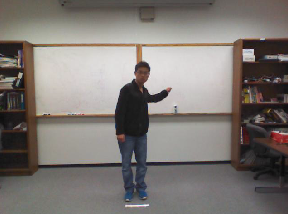
\includegraphics[scale=0.4]{tennis_swing.png}
\end{center}
\caption{\label{fig:tennis_swing_vid} Video dataset of a subject performing a tennis swing}
\end{figure}
In this paper, we would only be using the inertial and skeleton dataset for our models. We split the train-validation data in the same fashion as the original paper \cite{UTD-MHAD}, where subjects 1, 3, 5, 7 would be used for training and subjects 2, 4, 6, 8 for validation, so that we could perform a baseline comparison.  
\subsection{Data Pre-processing}
\subsubsection{Inertial Data}
The inertial data was re-sampled to the mean period of $180$ units. This was found to allow the model to achieve convergence much quicker. Amplitude normalization was also tried but subsequently removed as it does not show improvement in the model's training. A histogram plot of the period distribution is shown in Fig. \ref{fig:period_hist}

\begin{figure}[H]
\begin{center}
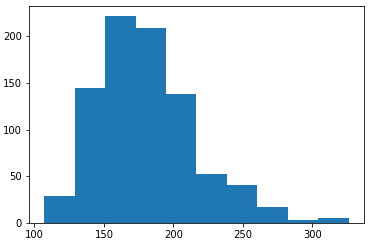
\includegraphics[scale=0.4]{period_hist.png}
\end{center}
\caption{\label{fig:period_hist} 
Histogram plot of the period distribution of Inertial Data}
\end{figure}
Histogram plots of the inertial data are shown in Fig. \ref{fig:amp_max_acc} - \ref{fig:amp_min_gyro} to show the distribution of amplitude for both maximum and minimum of the 3-axial accelerometer and gyroscope.
\begin{figure}[H]
\begin{center}
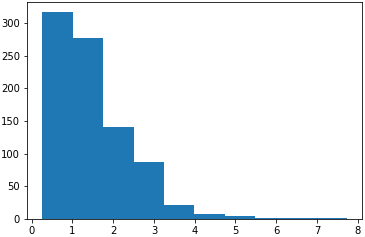
\includegraphics[scale=0.4]{amp_max_acc_hist.png}
\end{center}
\caption{\label{fig:amp_max_acc} 
Histogram plot of the period distribution of the maximum amplitude of the 3-axial accelerometer data}
\end{figure}
\begin{figure}[H]
\begin{center}
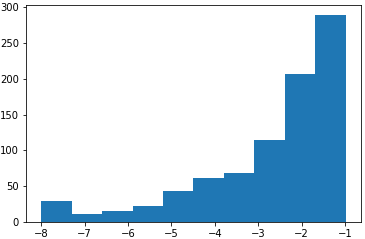
\includegraphics[scale=0.4]{amp_min_acc_hist.png}
\end{center}
\caption{\label{fig:amp_min_acc} 
Histogram plot of the period distribution of the minimum amplitude of the 3-axial accelerometer data}
\end{figure}
\begin{figure}[H]
\begin{center}
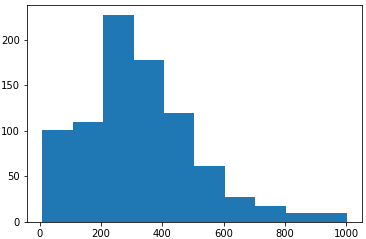
\includegraphics[scale=0.4]{amp_max_gyro_hist.png}
\end{center}
\caption{\label{fig:amp_max_gyro} 
Histogram plot of the period distribution of the maximum amplitude of the 3-axial gyroscope data}
\end{figure}
\begin{figure}[H]
\begin{center}
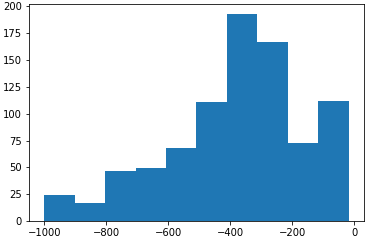
\includegraphics[scale=0.4]{amp_min_gyro_hist.png}
\end{center}
\caption{\label{fig:amp_min_gyro} 
Histogram plot of the period distribution of the minimum amplitude of the 3-axial gyroscope data}
\end{figure}
\subsubsection{Skeleton Data}
To aid with data fusion later, we re-sampled the skeleton data having $180$ frames. 
\subsection{Models}
For all our models, we used the AdamOptimizer \cite{Adam} with a learning rate of $1e^{-4}$, $\beta_1$ of $0.9$, and $\beta_2$ of $0.999$. We initialize our trainable parameters using the Xavier Glorot initializer \cite{GlorotB10}, and set our batch size to $3$ to allow our model our model to generalize better \cite{HofferHS17}. In this paper, we shall experiment with the following models: 
\begin{enumerate}
\item Simple LSTM
\item BiDirectional LSTM
\item Conv LSTM
\item UNet LSTM
\item Ensemble of Conv LSTM and UNet LSTM
\end{enumerate}
\vspace{0.5cm}
The full architecture of the models can be found in the Appendix.
\subsubsection{Simple LSTM}
We start off by having a Simple LSTM model, which comprises of an LSTM unit of $512$ hidden units, followed by a Dense layer, to classify all 27 actions. The LSTM \cite{LSTM} uses a gated approach to learn local, distributed, real-valued, and noisy pattern representations much quicker then real-time recurrent learning, back propagation through time, recurrent cascade correlation, Elman nets, and neural sequence chunking. Each recurrent unit in the LSTM was set to have a dropout rate of $0.2$.\\ \\
\subsubsection{BiDirectional}
The next model flips the copy of LSTM unit and concatenates it with original LSTM unit. This allows a form of generative deep learning, where the output layer can get information from the backwards and forward states simultaneously \cite{bidirectionalrecurrent}. This is then followed by a Dense layer with a softmax activation, to classify all 27 actions.\\ \\
\subsubsection{Conv LSTM}
The third model uses a series of 1D Convolutional and 1D Maxpooling layers to extract higher dimensional features before feeding them into $2$ LSTM units to capture the temporal information. The output of the LSTM units is then flattened out and we attached a Dropout layer with a dropout rate of $0.5$ before adding a Dense layer with a softmax activation to classify all 27 actions.\\ \\
\subsubsection{UNet LSTM}
The last model is adapted from a popular architecture commonly used in image semantic segmentation tasks. The UNet \cite{UNet} is an encoder-decoder convolutional neural network that is almost symmetric in the contraction and expansion path. In the contraction path, the input was is being fed through a series of convolutions and max-pooling, increasing the feature maps and decreasing the resolution of the image. This increases the ``what" and decreases the ``where". In the expansion path, the high dimensional features with low resolution is being up-sampled via convolutional kernels. The features maps were reduced during this operation. A novel feature of UNet is that it implements a concatenation of high dimensional features in the contraction path to the low dimensional feature maps of the expansion layers.\\ \\
\subsubsection{Ensemble of Conv LSTM and UNet LSTM}
The Conv LSTM and UNet LSTM were found to be performing well on the validation set, so we took an average of their softmax activation to create an ensemble as shown below.
\begin{equation}
\sigma(z)_{j, ensemble} = \frac{\sigma(z)_{j, cLSTM} + \sigma(z)_{j, uLSTM}}{2}
\end{equation}
where $\sigma(z)_j$ is the softmax output for an action $j$, given by:
\begin{equation}
\sigma(z)_j = \frac{\exp(z_j)}{\sum^{27}_{k=1} \exp (z_k)}
\end{equation}
\section{Computational Simulation}
The code is written in Python, using Keras with Tensorflow backend, NumPy, SciPy and Matplotlib libraries. The code can be found in this Github repository, \url{https://github.com/notha99y/Multimodal\_human\_actions}. The models are trained on Google Colaboratory notebooks.
\section{Results}
\subsection{Inertial Data}
\subsubsection{Simple LSTM}
The accuracy on the validation of our simple LSTM was $0.238$. The train-val accuracy and loss plots of the Simple LSTM are shown in Fig. \ref{fig:train_val_acc_simple_LSTM}, \ref{fig:train_val_loss_simple_LSTM} respectively. It shows that the model is quickly over-fitting after epoch $2$. The confusion matrix is show in Fig. \ref{fig:confusion_matrix_simple_LSTM}. 
\begin{figure}[H]
\begin{center}
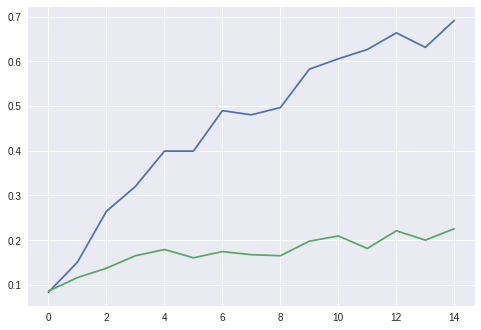
\includegraphics[scale=0.4]{simple_LSTM/simpleLSTM_acc_plot.png}
\end{center}
\caption{\label{fig:train_val_acc_simple_LSTM} 
Train (blue)-val (green) accuracy plot of the Simple LSTM model}
\end{figure}
\begin{figure}[H]
\begin{center}
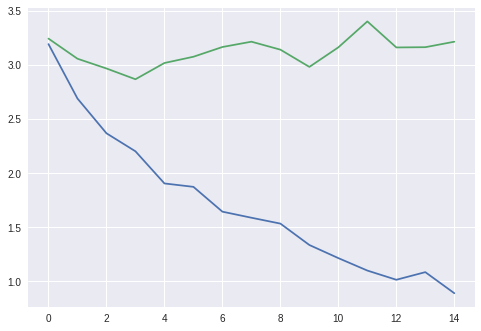
\includegraphics[scale=0.4]{simple_LSTM/simpleLSTM_loss_plot.png}
\end{center}
\caption{\label{fig:train_val_loss_simple_LSTM} 
Train (blue)-val (green) loss plot of the Simple LSTM model}
\end{figure}
\begin{figure}[H]
\begin{center}
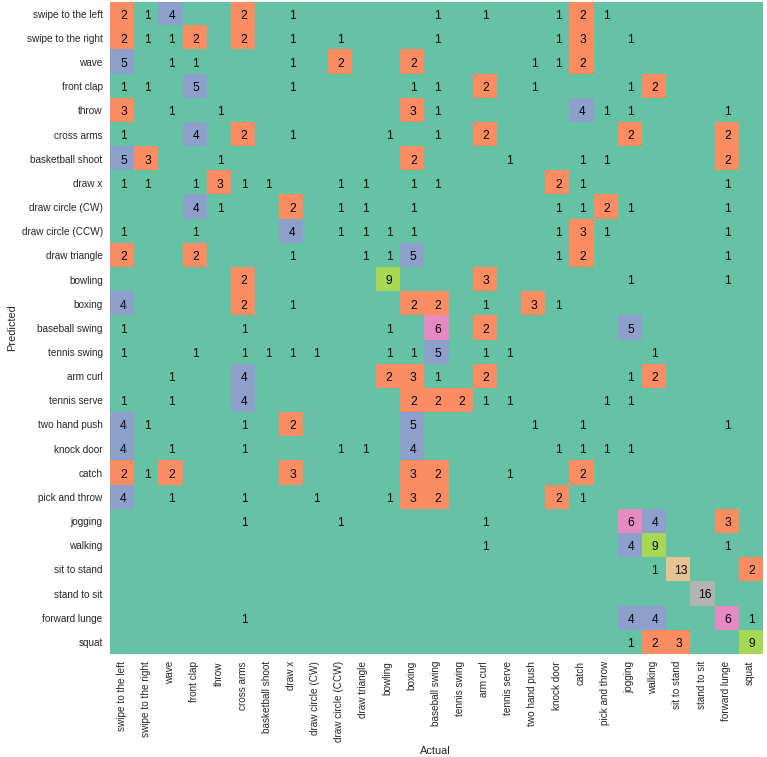
\includegraphics[scale=0.3]{simple_LSTM/simpleLSTM_confusion_matrix.png}
\end{center}
\caption{\label{fig:confusion_matrix_simple_LSTM} 
Confusion matrix of the Simple LSTM model}
\end{figure}
\subsubsection{Bi-Directional LSTM}
Similarly, the train-val accuracy, loss plots are shown in in Fig.\ref{fig:train_val_acc_bidirectional_LSTM}, \ref{fig:train_val_loss_bidirectional_LSTM} respectively, with the confusion matrix in Fig. \ref{fig:confusion_matrix_bidirectional_LSTM} with a validation accuracy of $0.465$.
\begin{figure}[H]
\begin{center}
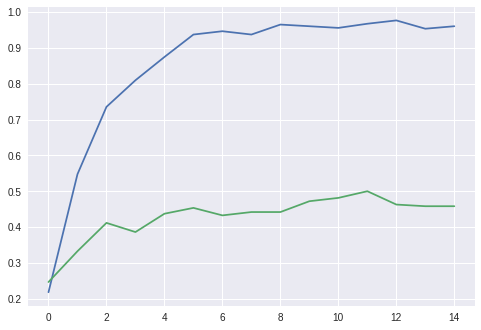
\includegraphics[scale=0.4]{bidirectional_LSTM/bidirectionalLSTM_acc_plot.png}
\end{center}
\caption{\label{fig:train_val_acc_bidirectional_LSTM} 
Train (blue)-val (green) accuracy plot of the Bi-Directional LSTM model}
\end{figure}
\begin{figure}[H]
\begin{center}
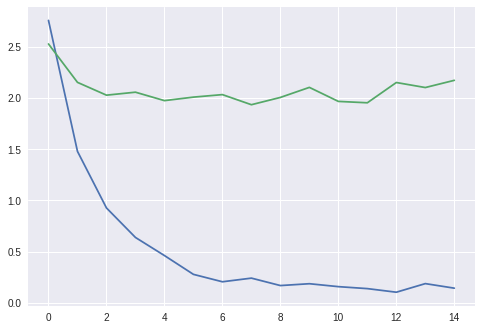
\includegraphics[scale=0.4]{bidirectional_LSTM/bidirectionalLSTM_loss_plot.png}
\end{center}
\caption{\label{fig:train_val_loss_bidirectional_LSTM} 
Train (blue)-val (green) loss plot of the Bi-Directional LSTM model}
\end{figure}
\begin{figure}[H]
\begin{center}
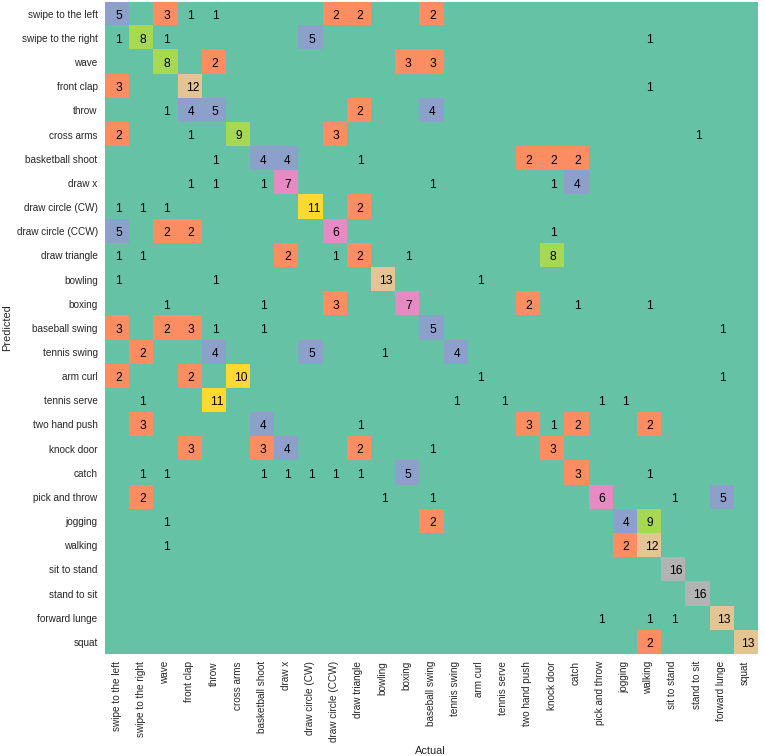
\includegraphics[scale=0.3]{bidirectional_LSTM/bidirectional_confusion_matrix.png}
\end{center}
\caption{\label{fig:confusion_matrix_bidirectional_LSTM} 
Confusion matrix of the Bi-Directional LSTM model}
\end{figure}

\subsubsection{Conv LSTM}
The Conv LSTM was the first major breakthrough among our models, achieving a validation accuracy of $0.700$. The train-val accuracy, loss plots are shown in Fig. \ref{fig:train_val_acc_conv_LSTM}, \ref{fig:train_val_loss_conv_LSTM} with the confusion matrix in Fig.
\ref{fig:confusion_matrix_conv_LSTM}.
\begin{figure}[H]
\begin{center}
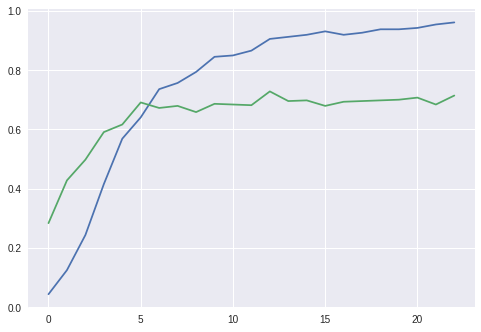
\includegraphics[scale=0.4]{conv_LSTM/conv_LSTM_acc_plot.png}
\end{center}
\caption{\label{fig:train_val_acc_conv_LSTM} 
Train (blue)-val (green) accuracy plot of the Conv LSTM model}
\end{figure}
\begin{figure}[H]
\begin{center}
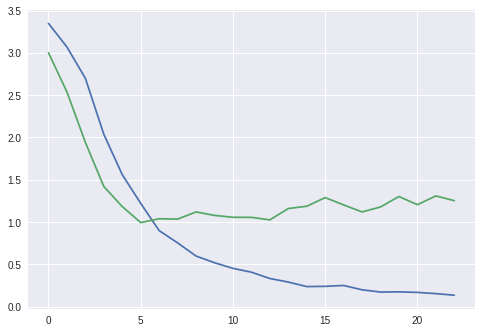
\includegraphics[scale=0.4]{conv_LSTM/conv_LSTM_loss_plot.png}
\end{center}
\caption{\label{fig:train_val_loss_conv_LSTM} 
Train (blue)-val (green) loss plot of the Conv LSTM model}
\end{figure}
\begin{figure}[H]
\begin{center}
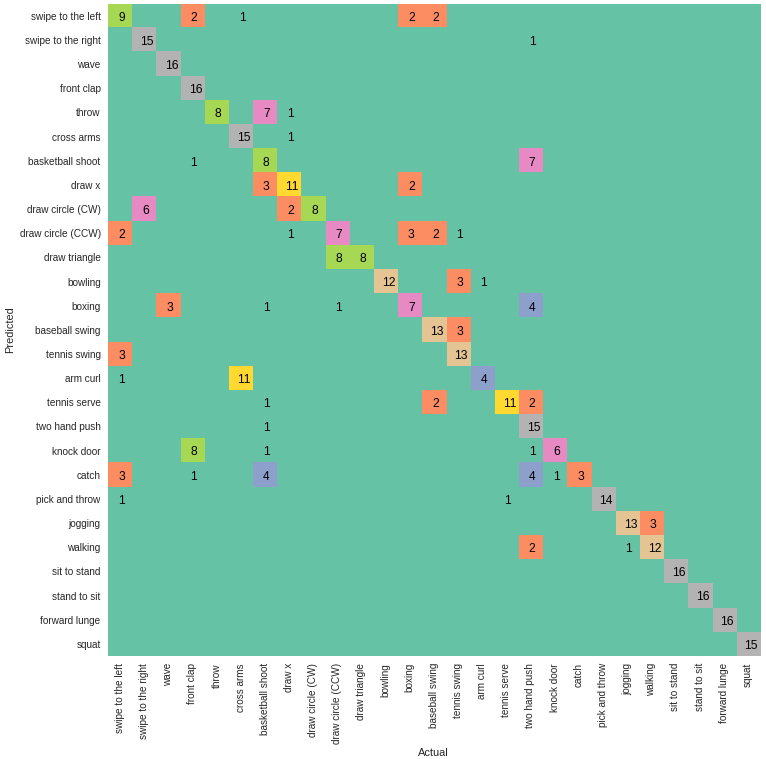
\includegraphics[scale=0.3]{conv_LSTM/conv_lstm_confusion_matrix.png}
\end{center}
\caption{\label{fig:confusion_matrix_conv_LSTM} 
Confusion matrix of the Conv LSTM model}
\end{figure}

\subsubsection{UNet LSTM}
Lastly, our UNet LSTM got the highest accuracy of $0.712$. The relevant plots are shown below.

\begin{figure}[H]
\begin{center}
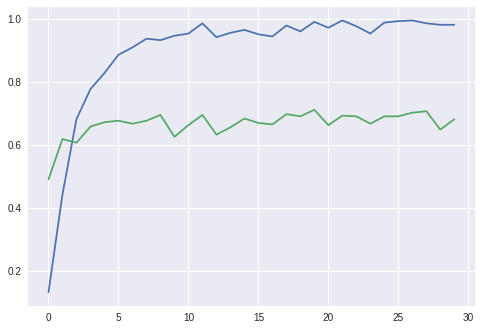
\includegraphics[scale=0.4]{UNet_LSTM/UNet_LSTM_acc_plot.png}
\end{center}
\caption{\label{fig:train_val_acc_UNet_LSTM} 
Train (blue)-val (green) accuracy plot of the UNet LSTM model}
\end{figure}
\begin{figure}[H]
\begin{center}
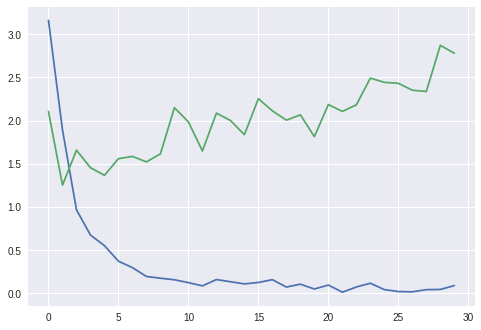
\includegraphics[scale=0.4]{UNet_LSTM/UNet_LSTM_loss_plot.png}
\end{center}
\caption{\label{fig:train_val_loss_UNet_LSTM} 
Train (blue)-val (green) loss plot of the UNet LSTM model}
\end{figure}
\begin{figure}[H]
\begin{center}
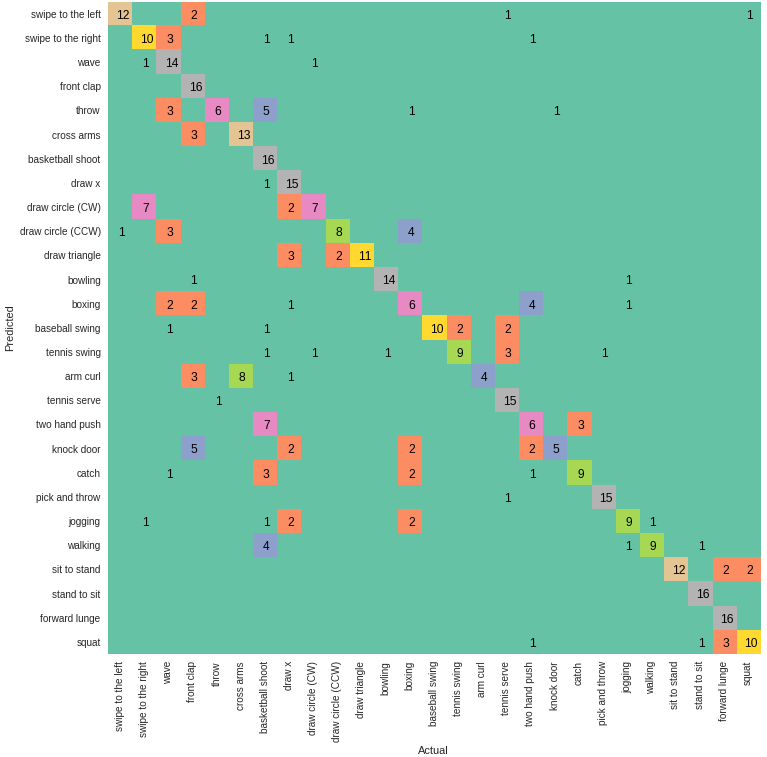
\includegraphics[scale=0.3]{UNet_LSTM/UNet_lstm_confusion_matrix.png}
\end{center}
\caption{\label{fig:confusion_matrix_UNet_LSTM} 
Confusion matrix of the UNet LSTM model}
\end{figure}
\subsubsection{Ensemble of Conv LSTM and UNet LSTM}
The confusion matrix of the ensemble is shown in Fig. \ref{fig:confusion_matrix_ensemble} with a total accuracy of $0.765$.
\begin{figure}[H]
\begin{center}
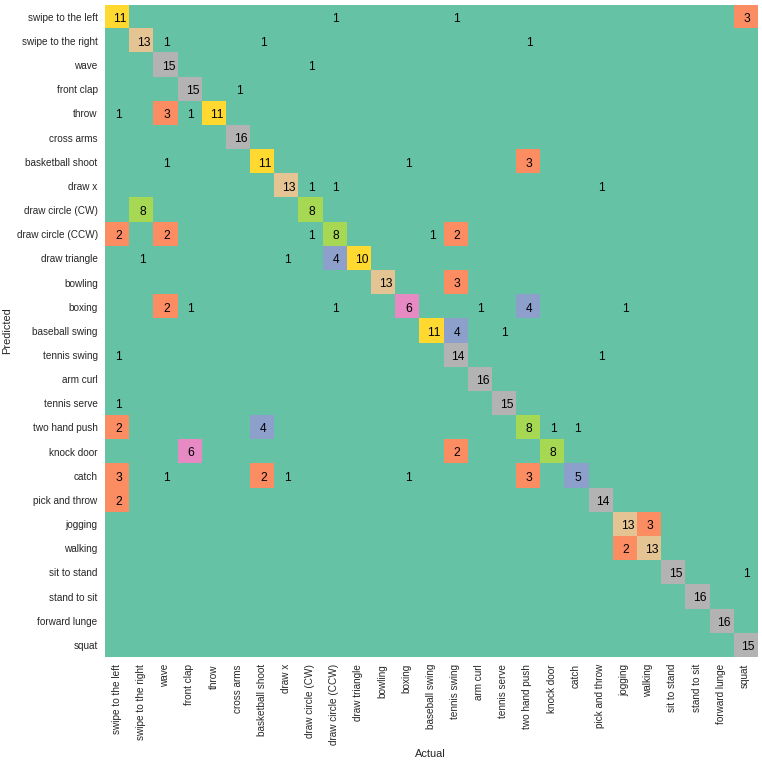
\includegraphics[scale=0.3]{ensemble_conv_UNet_LSTM/ensemble_conv_UNet_lstm_confusion_matrix.png}
\end{center}
\caption{\label{fig:confusion_matrix_ensemble} 
Confusion matrix of the Ensemble of Conv LSTM and UNet LSTM}
\end{figure}

\subsection{Inertial + Skeleton Data}
\subsubsection{Conv LSTM}
We combined the Skeleton data along the features axis with the Inertial data and trained the Conv LSTM to achieve an accuracy of $0.784$. The train-val accuracy, loss plots together with the confusion matrix is shown below.
\begin{figure}[H]
\begin{center}
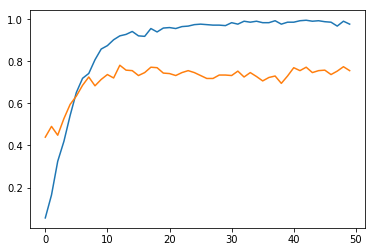
\includegraphics[scale=0.4]{conv_LSTM_iner_skel/conv_LSTM_acc_plot_iner_skel.png}
\end{center}
\caption{\label{fig:train_val_acc_conv_LSTM_iner_skel} 
Train (blue)-val (green) accuracy plot of the Conv LSTM model on both Inerital and Skeleton Data}
\end{figure}
\begin{figure}[H]
\begin{center}
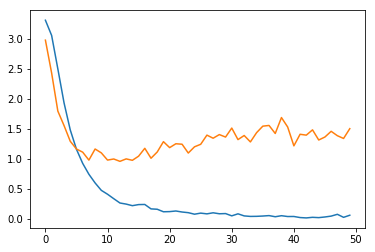
\includegraphics[scale=0.4]{conv_LSTM_iner_skel/conv_LSTM_loss_plot_iner_skel.png}
\end{center}
\caption{\label{fig:train_val_loss_conv_LSTM_iner_skel} 
Train (blue)-val (green) loss plot of the Conv LSTM model on both Inerital and Skeleton Data}
\end{figure}
\begin{figure}[H]
\begin{center}
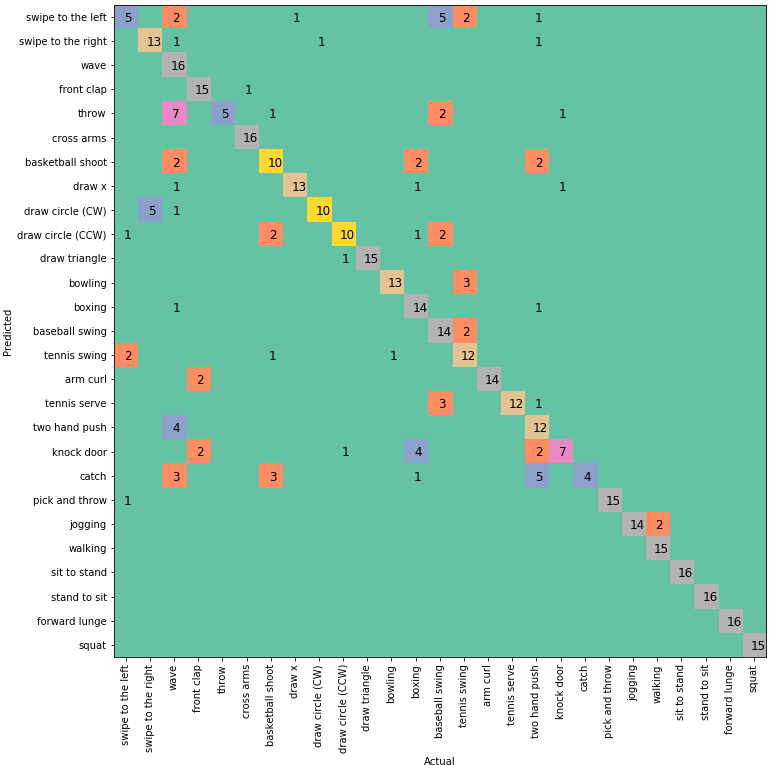
\includegraphics[scale=0.3]{conv_LSTM_iner_skel/conv_lstm_confusion_matrix_iner_skel.png}
\end{center}
\caption{\label{fig:confusion_matrix_conv_LSTM_iner_skel} 
Confusion matrix of the Conv LSTM model on both Inerital and Skeleton Data}
\end{figure}
\subsubsection{UNet LSTM}
Similiarly, the same was done with the UNet LSTM model and it achieve an accuracy of $0.742$. The relevant plots are shown below.
\begin{figure}[H]
\begin{center}
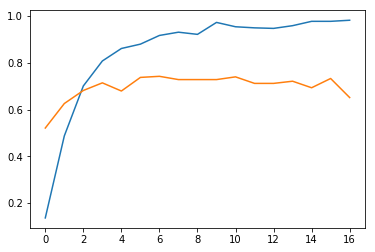
\includegraphics[scale=0.4]{UNet_LSTM_iner_skel/UNet_LSTM_acc_plot_iner_skel.png}
\end{center}
\caption{\label{fig:train_val_acc_UNet_LSTM_iner_skel} 
Train (blue)-val (green) accuracy plot of the UNet LSTM model on both Inertial and Skeleton Data}
\end{figure}
\begin{figure}[H]
\begin{center}
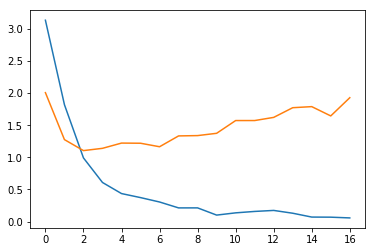
\includegraphics[scale=0.4]{UNet_LSTM_iner_skel/UNet_LSTM_loss_plot_iner_skel.png}
\end{center}
\caption{\label{fig:train_val_loss_UNet_LSTM_iner_skel} 
Train (blue)-val (green) loss plot of the UNet LSTM model on both Inertial and Skeleton Data}
\end{figure}
\begin{figure}[H]
\begin{center}
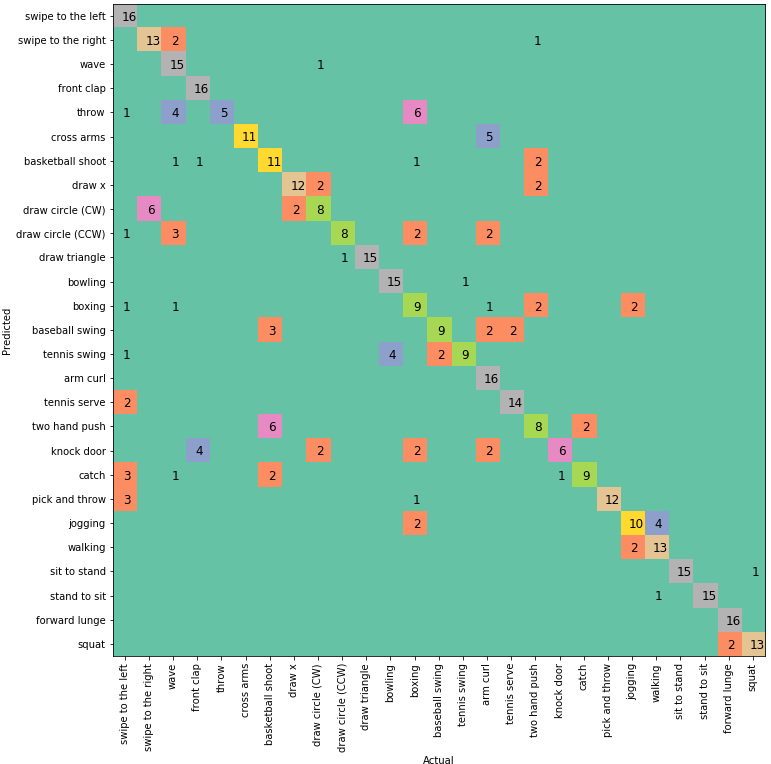
\includegraphics[scale=0.3]{UNet_LSTM_iner_skel/UNet_lstm_confusion_matrix_iner_skel.png}
\end{center}
\caption{\label{fig:confusion_matrix_UNet_LSTM_iner_skel} 
Confusion matrix of the UNet LSTM model on both Inertial and Skeleton Data}
\end{figure}
\subsubsection{Ensemble of Conv LSTM and UNet LSTM}
Lastly, we combined all our stocks together and put together an ensemble which achieved an accuracy of $0.821$. The confusion matrix is shown below in Fig \ref{fig:confusion_matrix_ensemble_iner_skel}.
\begin{figure}[H]
\begin{center}
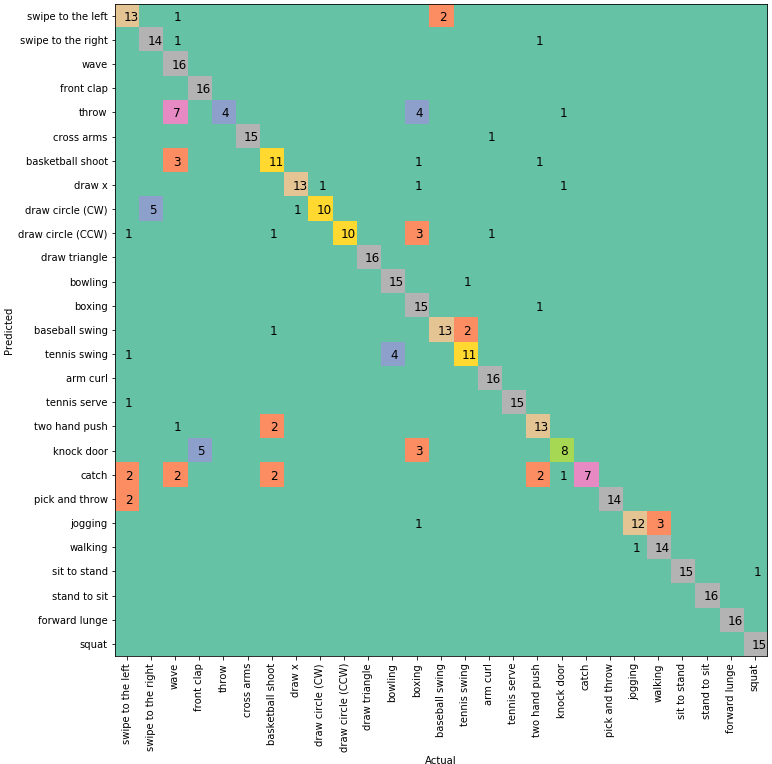
\includegraphics[scale=0.3]{ensemble_conv_UNet_LSTM/ensemble_UNet_lstm_confusion_matrix_iner_skel.png}
\end{center}
\caption{\label{fig:confusion_matrix_ensemble_iner_skel} 
Confusion matrix of the Ensemble of Conv LSTM and UNet LSTM model on both Inertial and Skeleton Data}
\end{figure}

\subsection{Summary}
The summary of results can be found below in Table. \ref{tbl:results_summary}. 
\begin{table}[H] 
\caption{Summary of validation accuracy of the different models} \label{tbl:results_summary}
\begin{tabular}{|c|c|c|c|c|c|}
\hline
& S-LSTM & B-LSTM & C-LSTM & U-LSTM & Ensemble \\
\hline
Iner & $0.238$ & $0.465$ & $0.700$ & $0.712$ & $0.765$ \\
\hline
Iner + skel & - & - & $0.784$ & $0.742$ & $0.821$ \\
\hline
\end{tabular}
\end{table}
\section{Discussion, and Conclusion}
In this paper, we have demonstrated an ensemble approach in HAR, achieving an accuracy of $0.821$ on the validation set using the Inertial and Skeleton Data which is an improvement compared to the baseline paper of $0.672$. This could be due to the convolutional networks being able to capture more generic, higher dimensional features compared to the Collaborative Representation Classifier (CRC) method used in \citep{1238378}-MHAD}. However, we find that there are still some things we can work on and in the following sub sections, we shall explore other methods as future work to improve our validation accuracy. 
\subsection{Issue of model over-fitting}
The main recurring challenge we faced was that our model was over-fitting at early epochs. Adding dropout layers seemed to reduce this, and ensembling the UNet LSTM with the Conv LSTM allows the our model to explore other solution spaces \cite{abs-1106-0257}. Over-fitting tends to happen when our model tries to learn high frequency features that may not be useful. Adding Gaussian Noise with zero mean and data points in all frequencies might enhance the learning capability of our model. Similarly, the time sequences of different subjects are quite varied even for the same activities. Performing data augmentation using time scaling and translation would increase the amount of training data, allowing our model to generalize better. On a side note, our model could also be trimmed further to reduce its complexity, and also its risk of over-fitting.
\subsection{Data Fusion of Depth and RGB data}
Fusion with the Depth and RGB data would allow more training input variables for our models to learn from, hence improving our validation accuracy. 
\subsection{Ensemble Learning}
Right now, our ensemble simply takes the average of our models’ softmax activations. We could further enhance the validation accuracy and reduce over-fitting, by exploring different ensemble learning approaches \cite{ensembleML} such as Boosting \cite{boosting}, Voting and Bagging mechanisms \cite{weaklearnability}. 
\section{Appendix}
\begin{figure}[H]
\begin{center}
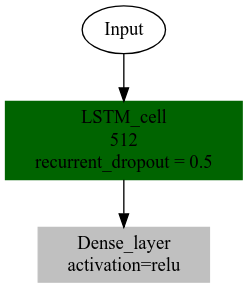
\includegraphics[scale=0.5]{models/simple_LSTM.png}
\end{center}
\caption{Full model of Simple LSTM}
\end{figure}
\begin{figure}[H]
\begin{center}
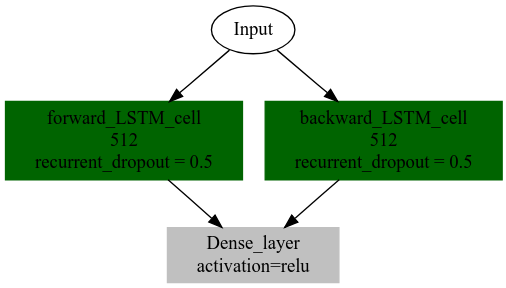
\includegraphics[scale=0.5]{models/bidirectional_LSTM.png}
\end{center}
\caption{Full model of Bi-Directional LSTM}
\end{figure}
\begin{figure}[H]
\begin{center}
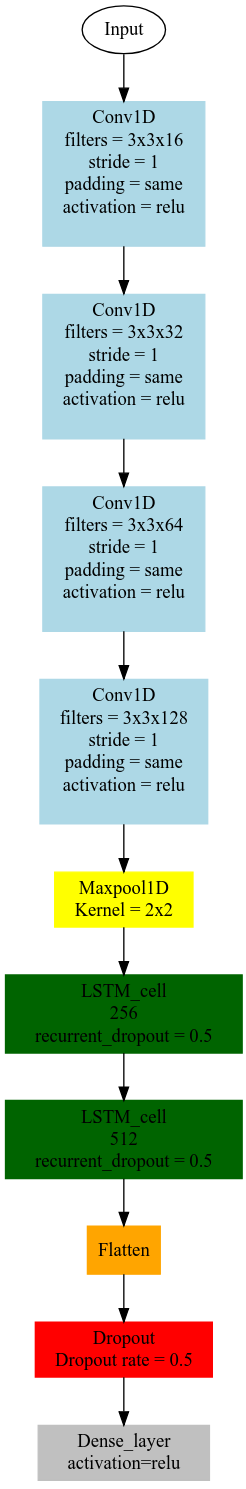
\includegraphics[scale=0.4]{models/conv_LSTM.png}
\end{center}
\caption{Full model of Conv LSTM}
\end{figure}
\begin{figure}[H]
\begin{center}
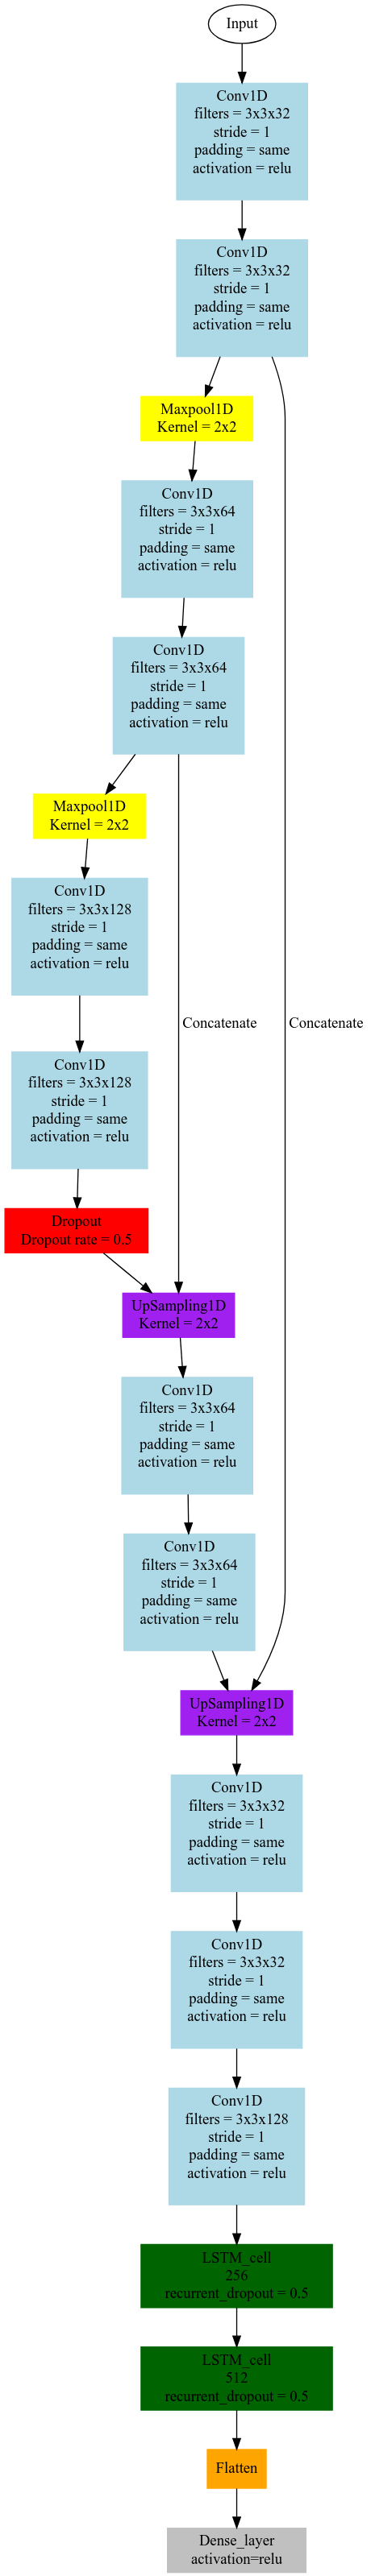
\includegraphics[scale=0.22]{models/UNet_LSTM.png}
\end{center}
\caption{Full model of UNet LSTM}
\end{figure}

\bibliographystyle{IEEEtran}
\bibliography{bibfile}
\end{document}
